\documentclass{anstrans}
%%%%%%%%%%%%%%%%%%%%%%%%%%%%%%%%%%%
\title{Evidence of the necessity of isotopic precise calculation in fuel cycle
calculation}
\author{Baptiste Mouginot$^{*}$, Paul P.H. Wilson$^{*}$, Robert W. Carlsen$^{*}$, Meghan B. McGarry$^{*}$,
Arrielle C. Opotowsky$^{*}$ }

\institute{
$^{*}$University of Wisconsin-Madison, WI
\and
%$^{\dagger}$State Capitol Building, Springfield, IL
}

\email{mouginot@wisc.edu \and paul.wilson@wisc.edu}

% Optional disclaimer: remove this command to hide
%\disclaimer{Notice: this manuscript is a work of fiction. Any resemblance to
%actual articles, living or dead, is purely coincidental.}

%%%% packages and definitions (optional)
\usepackage{graphicx} % allows inclusion of graphics
\usepackage{booktabs} % nice rules (thick lines) for tables
\usepackage{microtype} % improves typography for PDF

\newcommand{\SN}{S$_N$}
\renewcommand{\vec}[1]{\bm{#1}} %vector is bold italic
\newcommand{\vd}{\bm{\cdot}} % slightly bold vector dot
\newcommand{\grad}{\vec{\nabla}} % gradient
\newcommand{\ud}{\mathop{}\!\mathrm{d}} % upright derivative symbol

\begin{document}
%%%%%%%%%%%%%%%%%%%%%%%%%%%%%%%%%%%%%%%%%%%%%%%%%%%%%%%%%%%%%%%%%%%%%%%%%%%%%%%%
\section{Introduction} 

The purpose of this study is to examine the importance of the isotopic
composition of plutonium on PWR MOX fuel fabrication as part of a multi-tiered
fuel cycle, and the effect of its evolution during a transition. Two main
effects can modify the isotopic composition of the plutonium used to build the
PWR-MOX fuel: decay and depletion.

This analysis is based on a transition of the nuclear fuel cycle
to a configuration identified as ``Evaluation Group 29'' or ``EG29'', in the
recently-published Evaluation and Screening (E\&S) report \cite{ES}.  The EG29 fuel
cycle corresponds to a double strata fleet. The first stratum is composed of
sodium-cooled fast reactors (SFRs) multi-recycling plutonium. Surplus
plutonium is sent to the second stratum composed of pressurized water
reactors with full mixed oxide (U/Pu)O$_{2}$ cores (MOX-PWRs).  The PWR stratum
is also multi-recycling its plutonium. The target energy generation ratio for
the final EG29 system is 70:30 (SFR:PWR), with a 1\% annual growth in nuclear
energy demand.

%% PPHW: Can we add the official FCDP images

All the calculation of this study have been performed using the Cyclus fuel cycle
tool\cite{CYCLUS}. The facility models are from the Cycamore package, developed by the
Cyclus team, and containing a Pu-equivalent fuel fabrication model as well as
a simple fixed mixing ratio fuel fabrication model. A new neural network model has
also been contributed to the Cyclus environment using the cyCLASS tool\cite{cyCLASS}, 
allowing the use of the fuel fabrication and depletion models from the CLASS tool
\cite{CLASS} in Cyclus.

%% PPHW: Need a reference to cyCLASS - perhaps tag a version and put a zip
%% file on figshare with a DOI.

\section{Study description}
This work compares the plutonium fraction required to build fresh MOX fuel
using three different stream mixing models in fuel fabrication: ``fixed mixing
ratio'', ``plutonium equivalent theory'', ``neural network'' \cite{CLASS_MLP}.
The first part of the study in focuses on the effect of decay on the isotopic
composition of the reprocessed plutonium and its impact on fuel fabrication
depending on the chosen stream mixing model.  The second part of the study,
compares the impact on fresh fuel compositions when used fuel is based on a
depletion calculation instead of a fixed recipe, using the neural network fuel
fabrication model, also including the impact of decay.


\subsection{Cycle}
This analysis is focused only on the second strata of EG29, represented by a single
PWR reactor using MOX fuel. After irradiation the uranium and the plutonium are
separated and reprocessed to fuel the next batch of MOX fuel for the PWR.
%% PPHW - must provide the separation parameters/efficiencies

\begin{figure}[ht] % replace 't' with 'b' to force it to be on the bottom
  \centering
  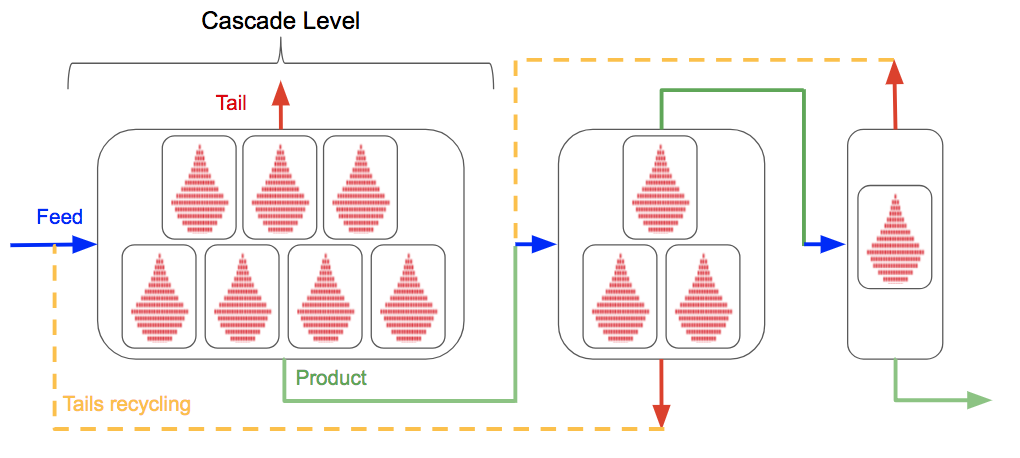
\includegraphics[width=0.48\textwidth]{flow}
  \caption{Schematic representation of the fuel cycle. Quantities next to arrows
  represent the cumulative amount (in kg) of material exchanged between two
facilities in the calculation using the ``pu-equivalent'' model for fuel fabrication, with decay activated.}
  \label{fig:flow}
\end{figure}

%% PPHW - must provide the composition of the ``good'' Pu
A stream of ``good'' quality plutonium coming from a hypothetical irradiated
SFR blanket is represented by a storage facility. 
%% PPHW - which facility?  which label - there are two.
The impact of the decay on this stored Pu
is limited, as the content in $^{241}$Pu is almost negligible.  In order to
build the first batch of fuel, an initial quantity of stored Pu has also been provided.
%% PPHW - how much?
In order to limit the effect of decay of this storage the initial inventory have been
tuned to be as small as possible, preventing any unnecessary accumulation of plutonium.
%% PPHW - is this about the initial inventory or the capacity of the storage facility
%%      - the latter seems to be about capacity

\subsection{Fabrication model}
Three different ways to model the fuel fabrication have been used: ``fix mixing
ratio'', ``Pu-equivalent'' and ``neural network''.
The fix mixing ratio is based on a user-defined ratio for the different stream mixing. The
``Pu-equivalent'' model finds the mixing ratio that results in an initial reactivity
that matches that of the requested MOX fuel recipe.  This ratio may change as the 
composition of the incoming streams changes.  As the requested fuel
composition corresponds to the fuel composition built with the ''fix mixing
ratio`` model, the results of those 2 models are expected to be similar.
The ``neural network'' model attempts to achieve a given reactivity at the end of a 
life for a given batch of fuel ($50~$GWd/t in this study). The
$<k_{infty}>$ used in this study is 1.034 \cite{???}. The neural network in this
model has been pre-trained on several different depletion calculations,
allowing it to predict the correct plutonium fraction required, depending
on the composition of that plutonium.

%% PPHW - is this end of cycle reactivity of the whole core for a multi-batch core?
%%      - or is it end of life reactivity for a given batch?
%%      - 1.034 and 50 GWd/t don't seem to go together

Because of these models have not necessary been tuned on exactly the same
PWR configuration and parameters, this analysis focuses on the differences
in the results due to the change in model rather than the results themselves.

The second part of the study compares the amount of plutonium require to build
the PWR-MOX fuel (using the neural network modeling for fuel fabrication) for
the recipe based output composition versus a compisition calculated by depletion.
To caluclate the depletion for each fuel batch loaded in the PWR reactor, another 
neural network is used to predict the macroscopic cross section of the
fuel \cite{NN_CLASS} (only fission, capture and n,2n reactions are considered). The
depletion calculation is done renormalizing the neutron flux to maintain a
constant power in the reactor.

%%%%%%%%%%%%%%%%%%%%%%%%%%%%%%%%%%%%%%%%%%%%%%%%%%%%%%%%%%%%%%%%%%%%%%%%%%%%%%%%
\section{Decay}

As observed in Fig. \ref{fig:nod}, despite the fact that the different models 
were not tuned to
describe the exact same PWR concept, the results without decay are very
close. They all predict a constant plutonium fraction around $8\%$ of plutonium
in the fresh PWR-MOX fuel.

\begin{figure}[ht] % replace 't' with 'b' to force it to be on the bottom
  \centering
  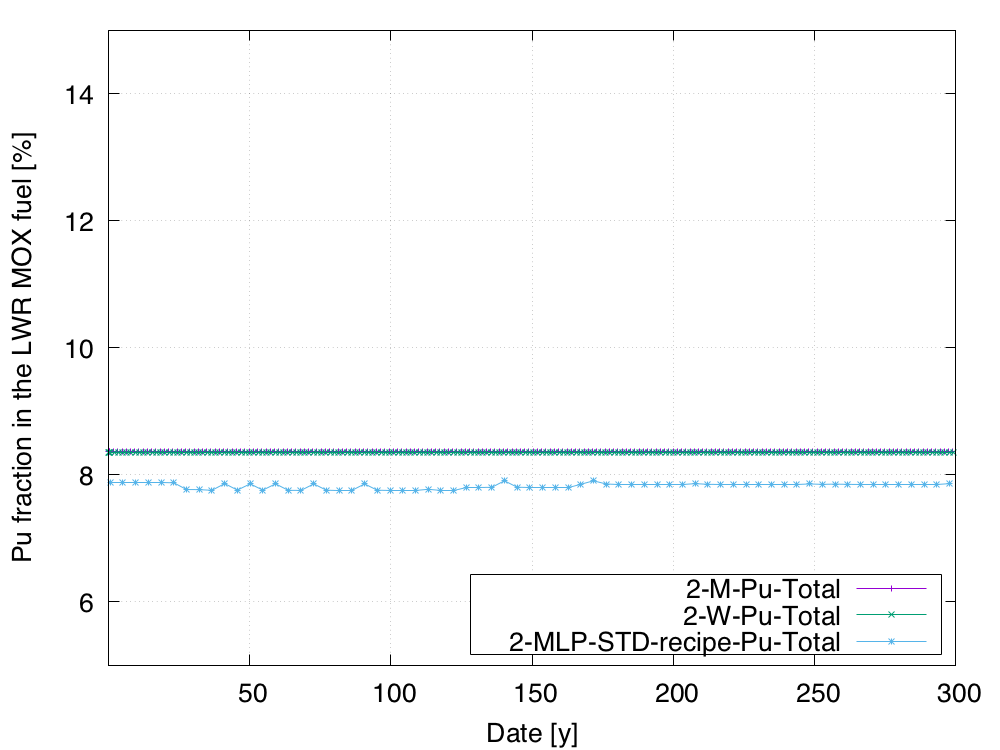
\includegraphics[width=0.48\textwidth]{nodecay_pu_contribution.png}
  \caption{Evolution of the fraction of plutonium in the fresh PWR-MOX fuel
    using 3 predicted models: fixed-mixing ratio, Pu-equivalent, and neural
    network (NN). Here decay is not considered, so the fixed-mixing ratio and Pu-equivalent models have the same evolution.}
  \label{fig:nod}
\end{figure}

%% PPHW - need better figure legend text so that readers know what they are
%% looking at
%% MBM - I only see two traces on the plot. If this is correct, then add the
%% following to the caption: `` The fixed stream and Pu-equivalent models have the same Pu fraction.''

With decay turned on, see Fig. \ref{fig:d}, results for the ``fix mixing ratio''
calculation see a small decrease of the fraction of plutonium in the fuel,
corresponding to the decay of $^{241}$Pu into $^{241}$Am.  For the
``Pu-equivalent'' modeling we can observe a slight increase of the fraction of
plutonium, which is required to compensate for the negative reactivity effect
coming from the $^{241}$Am. For the calculation using ``neural network'' fuel
fabrication modeling the effect is very quickly increasing to $13\%$ and then
slowing stabilizing as the plutonium composition approaches an equilibrium.

\begin{figure}[ht] % replace 't' with 'b' to force it to be on the bottom
  \centering
  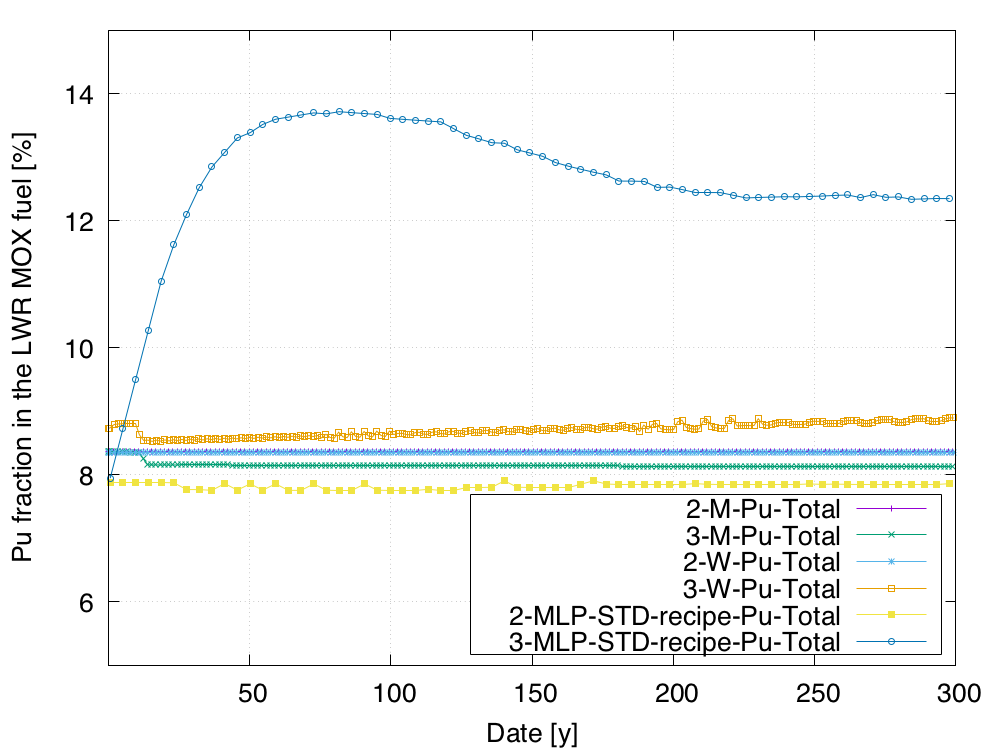
\includegraphics[width=0.48\textwidth]{decay_pu_contribution.png}
  \caption{Comparison of the effects of decay on
    evolution of the fraction of plutonium in the fresh PWR-MOX fuel
    using the 3 prediction models.  Solid line shows the Pu fraction over time
    without tracking decay. Dashed line of the same color shows the the
    same model, but with decay enabled. Decay has a particularly large effect
  on the neural network (NN) model.}
  \label{fig:d}
\end{figure}

%% PPHW - need better color and symbol choices to facilitate comparison
%%      - different models use different colors and decay/no decay uses
%%      -  different symbols (for example)

As the calculation using ``neural network'' fabrication modeling requires more
plutonium than the cycle can produce, the initial inventory has been set to a
higher values, increasing the plutonium decay effect. Nevertheless this shows
the strong impact of the presence of $^{241}$Am with the plutonium used for the
PWR-MOX fuel fabrication.

%% PPHW: why is the Pu-equiavlent model so bad?

A last calculation, on decay have been performed using the ``Pu-equivalent''
fabrication model, increasing by a factor 2, 5 and 10 the amount of plutonium in
the startup inventory.  This mimics different degrees of a plutonium accumulation,
and thus different impacts from the decay of this plutonium.
This calculation shows a change from 10 to 30\% in the mixing ratio required to
build the proper PWR-MOX fuel. This kind of plutonium accumulation can
unexpectedly occur in a real fuel cycle and might need to be considered in a
complete fuel cycle transition study.
%% PPHW - do you plot results for this?


The decay process tends to change to composition of the plutonium vector, and
then of the plutonium enrichment required to build a proper PWR-MOX fuel.  Such
composition change in the MOX fuel will impact the individual cross sections:
particularly in thermal reactors where the macroscopic cross sections are very
dependent on the shape of the thermal part of the neutron spectrum, which is
strongly driven by the fuel isotopic composition.


%%%%%%%%%%%%%%%%%%%%%%%%%%%%%%%%%%%%%%%%%%%%%%%%%%%%%%%%%%%%%%%%%%%%%%%%%%%%%%%%
\section{Depletion vs Recipe}

Another analysis was performed to evaluate the impact of the depletion
calculation on a fuel cycle macroscopic (???) level.

\begin{figure}[ht] % replace 't' with 'b' to force it to be on the bottom
  \centering
  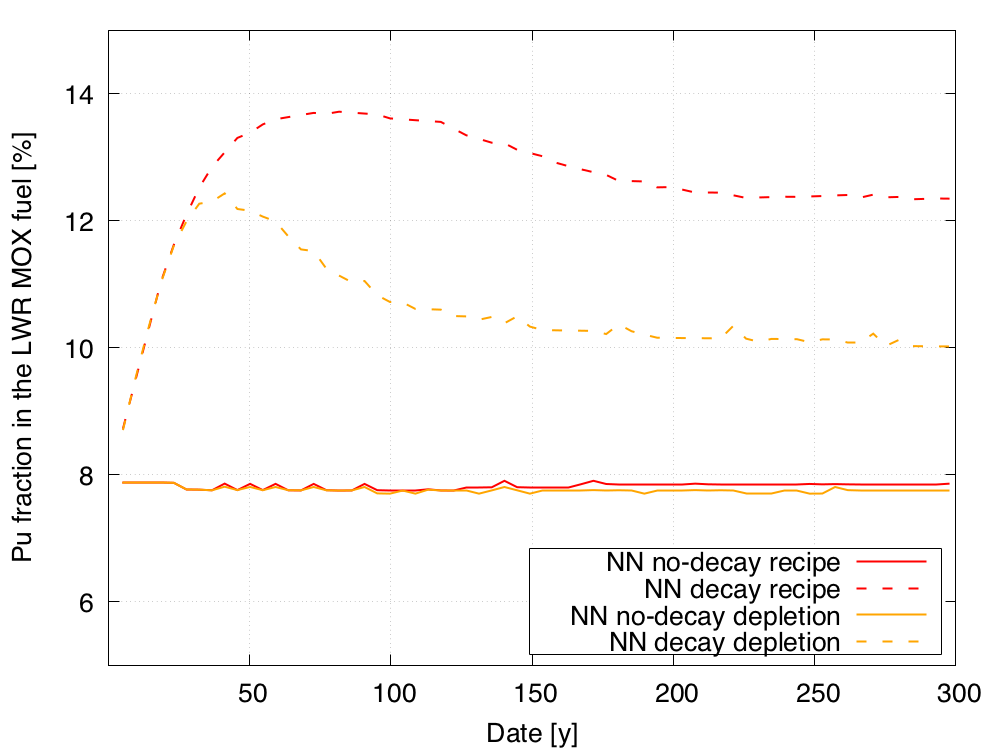
\includegraphics[width=0.48\textwidth]{irradiation_pu_contribution.png}
  \caption{Evolution of the fraction of plutonium in the fresh PWR-MOX fuel
    using four models utilizing a ``neural network''.  The solid red trace
    uses a reciped based model to define spent fuel composition, while the
    dashed red line also includes decay.  The orange traces compare the effects
    of decay while using a depletion model to dynamically recalculate spent
    fuel composition.}
  \label{fig:depletion}
\end{figure}

%% PPHW: - I don't know which answer is which !?!?  bad legend labels!

%% PPHW: I don't know what the difference between these calculations is!!!
%% You have 4 results but haven't made clear what the variations are. Do they
%% all have decay?  I think the following is correct, but I'm not sure...

Four simulations were carried out representing variations across two problem
dimensions.  One variation compares how reactor models determine the recipe of
used fuel.  The standard recipe reactor model produces used fuel of a fixed
composition, regardless of the composition of the incoming fuel.  The
alternative is a neural network depletion model provided by the cyCLASS
package.  This model determines the composition of the used fuel depending on
its initial composition and discharge burnup.  Both of these models were used
without decay and with decay.

As shown on Fig. \ref{fig:depletion}, the equilibrium values for recipe based
calculation and the depletion calculation are not the same. Moreover,
recalculating the fuel spent fuel composition for each fuel batch allows the
cycle to reach equilibrium faster.

This is caused by the slight change in the composition in the available plutonium
(see Fig. \ref{fig:depletioncompo}): in the case of the depletion calculation
the available plutonium contain $68\%$ of $^{239}$Pu versus $64\%$ in the recipe
based case, and also significantly less $^{241}$Pu leading to less $^{242}$Pu in
the cycle. The amounts of the other nuclides are very close.

\begin{figure}[ht] % replace 't' with 'b' to force it to be on the bottom
  \centering
  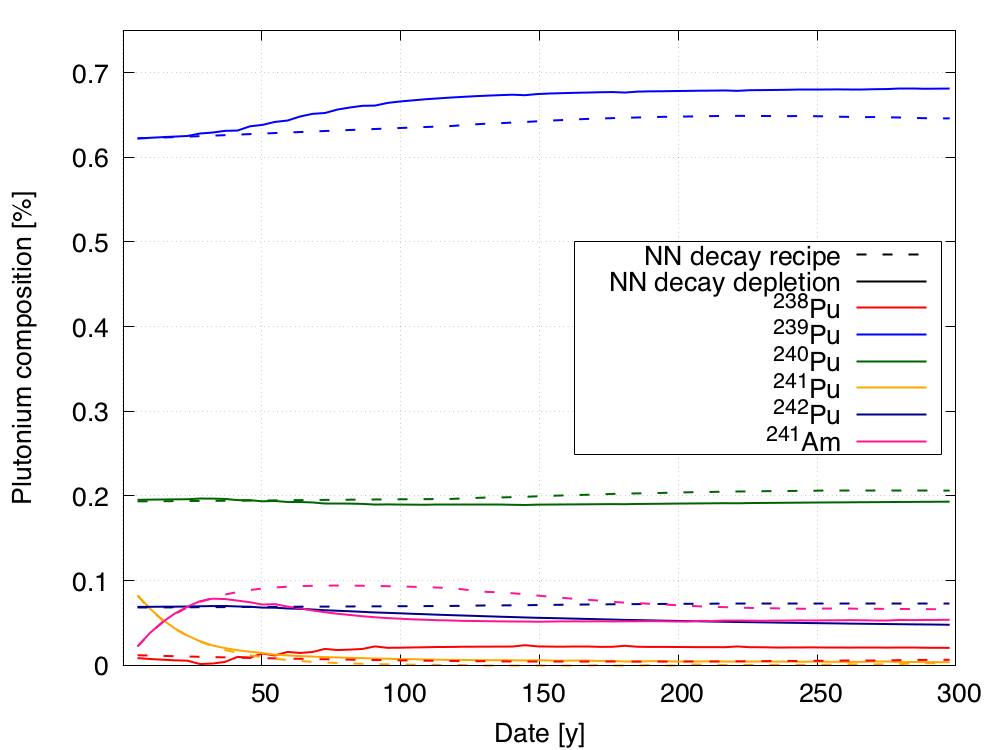
\includegraphics[width=0.48\textwidth]{MOX_pu_composition.png}
  \caption{Effects of the model used to define spent fuel composition on the evolution of representative isotopes in fresh PWR-MOX fuel
    using the ``neural network'' model, with decay activated. Dashed lines indicate the fraction of the
    istope present using a recipe based model for spent fuel. Solid lines of the same color indicate isotope fraction using the depletion model.}

  \label{fig:depletioncompo}
\end{figure}

Those slight change in the output composition, lead to an overall decrease in
the amount of $^{241}$Am in the fresh PWR-MOX fuel and an increase of the
$^{239}$Pu, allowing to build fuel with a lower plutonium enrichment.


%%%%%%%%%%%%%%%%%%%%%%%%%%%%%%%%%%%%%%%%%%%%%%%%%%%%%%%%%%%%%%%%%%%%%%%%%%%%%%%%
\section{Conclusions}

This study has shown the potential impact of the decay process on the MOX-PWR fuel
fabrication process, increasing the required amount from $1\%$ to $4\%$
depending on the fuel fabrication model choice. The recalculation of the 
depletion of each loaded fuel batch has consequences on the equilibrium
state of the calculation: the reduction of fraction of $^{241}$Am and the increase of the
fraction $^{239}$Pu in the available plutonium allows a reduction in the amount of
plutonium in the fuel.

This work has shown the strong influence of the isotopic composition on a LWR
cycle involving plutonium recycling. Similar analysis will be conducted in the
near future on the SFR strata of the EG29 fuel cycle, which should be less
impacted by those isotopic changes, as fast spectrum reactor are less sensitive
to those change.

Moreover this study has demonstrated the value of the modular design of
Cyclus, able to investigate differences between the physics fidelity of
facility models in an isolated fashion, with other fuel cycle components
unchanged.  In this case, additional fidelity was introduced rapidly by
wrapping the existing neural network models made available by CLASS.



%%%%%%%%%%%%%%%%%%%%%%%%%%%%%%%%%%%%%%%%%%%%%%%%%%%%%%%%%%%%%%%%%%%%%%%%%%%%%%%%
%\appendix
%\section{Appendix}
%
%Numbering in the appendix is different:
%\begin{equation} \label{eq:appendix}
%  2 + 2 = 5\,.
%\end{equation}
%and another equation:
%\begin{equation} \label{eq:appendix2}
%  a + b = c\,.
%\end{equation}

%%%%%%%%%%%%%%%%%%%%%%%%%%%%%%%%%%%%%%%%%%%%%%%%%%%%%%%%%%%%%%%%%%%%%%%%%%%%%%%%
\section{Acknowledgments}
Shall we acknowledge anyone ? DOE ? FCO ?


%%%%%%%%%%%%%%%%%%%%%%%%%%%%%%%%%%%%%%%%%%%%%%%%%%%%%%%%%%%%%%%%%%%%%%%%%%%%%%%%
\bibliographystyle{ans}
\bibliography{bibliography}
\end{document}

